\begin{prob}
For the following problems, recall that $(u, v)$ is a
\emph{tree edge} if node $v$ is discovered while visiting node $u$
during a breadth-first or depth-first search. Assume the convention
that a node's neighbors are produced in ascending order by label.
You do not need to show your work for this problem.


\newcommand{\drawgraph}{
    \foreach \i in {1,...,9}{
        \pgfmathparse{mod(\i-1,3)} \pgfmathresult %displays 2.0
        \pgfmathtruncatemacro{\x}{\pgfmathresult}  

        \pgfmathtruncatemacro{\y}{(\i-1)/3}

        \node[draw, circle] (n\i) at (2*\x, 2*\y) {$\i$}; 
    }

    \draw (n5) edge[] (n7);
    \draw (n4) edge[] (n5);
    \draw (n6) edge[] (n5);
    \draw (n5) edge (n8);
    \draw (n2) edge[] (n6);
    \draw (n6) edge[] (n9);
    \draw (n1) edge[] (n2);
    \draw (n1) edge[] (n4);
    \draw (n8) edge[] (n9);
    \draw (n2) edge[] (n3);
    \draw (n6) edge[] (n3);
    \draw (n2) edge[] (n4);
    \draw (n6) edge[] (n8);
}


\begin{subprobset}
    \begin{subprob}
        Suppose a breadth-first search is performed on the graph below,
        starting at node 1. Mark every BFS tree edge with a bold arrow
        emanating from the predecessor. 

        \begin{center}
            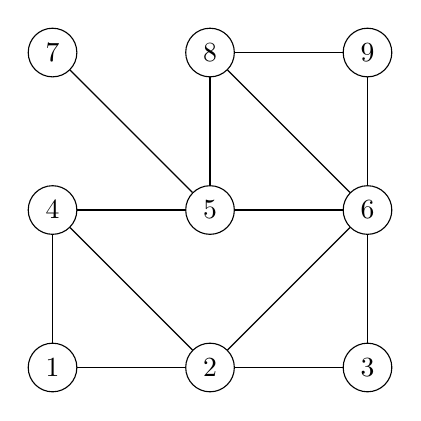
\begin{tikzpicture}
                \drawgraph{}
            \end{tikzpicture}
        \end{center}

        \begin{soln}

            % write your solution here
        \end{soln}

    \end{subprob}

    \begin{subprob}
        Suppose a depth-first search is performed on the graph below, starting
        at node 1. Mark every DFS tree edge with a bold arrow emanating from
        the predecessor. 

        \begin{center}
            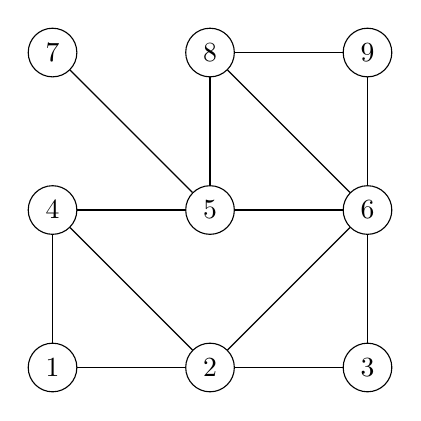
\begin{tikzpicture}
                \drawgraph{}
            \end{tikzpicture}
        \end{center}

        \begin{soln}

            % write your solution here
         \end{soln}
    \end{subprob}

    \begin{subprob}
        Fill in the table below so that it contains the start and
        finish times of each node after a DFS is performed on the above graph using node 1 as the source.
        Begin your start times with 1.

        \begin{center}
            \begin{tabular}{ccc}
                Node & Start & Finish\\
                % insert your answer in the braces.
                % e.g.:
                % 1 & \inlineresponsebox[.5in]{ 42 } & \inlineresponsebox[.5in]{ 99 } \\
                1 & \inlineresponsebox[.5in]{ } & \inlineresponsebox[.5in]{ } \\
                2 & \inlineresponsebox[.5in]{ } & \inlineresponsebox[.5in]{ } \\
                3 & \inlineresponsebox[.5in]{ } & \inlineresponsebox[.5in]{ } \\
                4 & \inlineresponsebox[.5in]{ } & \inlineresponsebox[.5in]{ } \\
                5 & \inlineresponsebox[.5in]{ } & \inlineresponsebox[.5in]{ } \\
                6 & \inlineresponsebox[.5in]{ } & \inlineresponsebox[.5in]{ } \\
                7 & \inlineresponsebox[.5in]{ } & \inlineresponsebox[.5in]{ } \\
                8 & \inlineresponsebox[.5in]{ } & \inlineresponsebox[.5in]{ } \\
                9 & \inlineresponsebox[.5in]{ } & \inlineresponsebox[.5in]{ } \\
            \end{tabular}
        \end{center}

        \begin{soln}
        % write your solution here
        \end{soln}
    \end{subprob}


\end{subprobset}

\end{prob}
